
%(BEGIN_QUESTION)
% Copyright 2006, Tony R. Kuphaldt, released under the Creative Commons Attribution License (v 1.0)
% This means you may do almost anything with this work of mine, so long as you give me proper credit

What is the response of this pneumatic relay to increasing pressure on each of its inputs?  Does the output pressure increase as input A's pressure increases?  What happens when input B's pressure increases?  Note that both the sensing and sealing diaphragms are welded to the pilot rod, forming leak-proof and frictionless seals between chambers:

$$\includegraphics[width=15.5cm]{i00198x01.eps}$$

Can you think of an electronic circuit or device that acts in an analogous manner?

\vskip 10pt

Also, explain why the following relay design is better, using two sealing diaphragms instead of just one.  A hint is to consider the {\it common-mode rejection} capacity of each relay design.  Once again, each of the metal diaphragms is welded to the rod to form leak-proof and frictionless seals:

$$\includegraphics[width=15.5cm]{i00198x03.eps}$$

\vskip 20pt \vbox{\hrule \hbox{\strut \vrule{} {\bf Suggestions for Socratic discussion} \vrule} \hrule}

\begin{itemize}
\item{} Explain how one might apply a ``thought experiment'' to these mechanisms to analyze their behavior.
\item{} Why use {\it sealing diaphragms} in mechanisms such as this?  Do you think there might be an alternative construction that achieves the same design goal?
\item{} Explain how the behavior of this relay is similar to that of an {\it operational amplifier}.  Which of the two inputs is the non-inverting (+) and which of the two is inverting ($-$)?
\end{itemize}

\underbar{file i00198}
%(END_QUESTION)





%(BEGIN_ANSWER)

A bit of explanation might be in order for the two diaphragms.  The larger diaphragm is called the {\it sensing} diaphragm, while the smaller diaphragm is called the {\it sealing} diaphragm.  The purpose of the sealing diaphragm is to prevent air pressure at input B from leaking out into the vented chamber just to the left of the wedge-shaped pilot plug.  This sealing diaphragm is made small enough that its contribution to force on the stem is negligible.  Only the sensing diaphragm is large enough to have any consequence upon the pilot valve's action.

\vskip 10pt

This is an equivalent electronic circuit:

$$\includegraphics[width=15.5cm]{i00198x02.eps}$$

%(END_ANSWER)





%(BEGIN_NOTES)

In this relay, the output pressure will tend to increase as input A pressure increases, and as input B pressure {\it decreases}.  In other words, input A is direct-acting (noninverting), and input B is reverse-acting (inverting).

\vskip 10pt

The operation of this device is not unlike a {\it differential amplifier} or an {\it operational amplifier}. 

\vskip 10pt

The second relay design is better because each input (A and B) has the exact same gain.  With the previous design, input A exhibits a greater gain than input B because any fluid pressure introduced to the ``B'' port presses against the sealing diaphragm in the opposite direction to the force exerted on the sensing diaphragm.  With two sealing diaphragms, {\it both} inputs have the equivalent effects on the sensing diaphragm.

%INDEX% Basics, pneumatics: relay action (direct vs. reverse)

%(END_NOTES)


